\chapter{Implementacija i korisničko sučelje}
		
		
		\section{Korištene tehnologije i alati}
		
			% \textbf{\textit{dio 2. revizije}}
			
			%  \textit{Detaljno navesti sve tehnologije i alate koji su primijenjeni pri izradi dokumentacije i aplikacije. Ukratko ih opisati, te navesti njihovo značenje i mjesto primjene. Za svaki navedeni alat i tehnologiju je potrebno \textbf{navesti internet poveznicu} gdje se mogu preuzeti ili više saznati o njima}.
			\noindent Projekt je izveden primjenom različitih tehnologija i alata u svrhu implementacije kao i za dokumentaciju. U nastavku slijedi lista alata i tehnologija koje smo koristili uz kratke opise njihove uporabe.
			\newline\newline
			\noindent\textbf{VisualStudioCode}\footnote[1]{https://code.visualstudio.com/} je besplatni visoko prilagodljiv tekstualni editor namijenjen širokom spektru programskih jezika i platformi. U sklopu ovoga projekta koristio se za pri pomoći u izradi dokumentacije. \textbf{LaTeX}\footnote[2]{https://www.latex-project.org/} je visokokvalitetan sustav za pisanje teksta koji se koristi za izradu tehničkih i znanstvenih dokumentacija zato što pruža konzistentan izgled dokumenta. Dokumentacija ovog projekta pisana je u LaTeX-u uporabom različitih okruženja kao što su \textbf{TeXStudio}\footnote[3]{https://www.texstudio.org/} (integrirano okruženje koje pruža sučelje za jednostavno pisanje, uređivanje i kompiliranje LaTeX koda), \textbf{Overleaf}\footnote[4]{https://www.overleaf.com/} (online suradnički editor koji omogućuje zajednički rad više korisnika na istom dokumentu u stvarnom vremenu) i \textbf{LaTeX Workshop}\footnote[5]{https://marketplace.visualstudio.com/items?itemName=James-Yu.latex-workshop} (extension unutar VSC-a koji pruža potpore za pisanje, uređivanje i kompiliranje LaTeX koda). Za izradu dijagrama korišten je \textbf{Astah}\footnote[6]{https://astah.net/} alat za modeliranje UML dijagrama. To je alat koji omogućuje vizualno prikazivanje struktura, interakcija i dinamike sustava što pomaže pri razumijevanju i planiranju arhitekture aplikacija. Također, dio dijagrama iscrtan je pomoću web-aplikacije za crtanje dijagrama \textbf{draw.io}\footnote[7]{https://app.diagrams.net/} koja pruža mogućnosti kao i Astah uz intuitivno korisničko sučelje koje olakšava vizualizaciju i komunikaciju ideja.
			\newline\newline
			\noindent\textbf{PostgreSQL}\footnote[8]{https://www.postgresql.org/} je snažan, open-source sustav za upravljanje bazama podataka koji podržava relacijski model podataka. Ova baza pruža napredne značajke poput transakcija, podrške za vanjske ključeve, indeksiranja i proširivosti. U ovome projektu PostgreSQL je korišten unutar integriranog razvojnog okruženja \textbf{DataGrip}\footnote[9]{https://www.jetbrains.com/datagrip/} koji nudi napredne alate uz brzu navigaciju, pisanje i testiranje SQL upita, upravljanje shemama i izvođenje drugih zadataka nad bazom podataka. Od ponuđenih administratorskih alata koristio se \textbf{pgAdmin4}\footnote[10]{https://www.pgadmin.org/download/} koji omogućuje korisnicima pregled i manipulaciju bazom, shemama, tablicama i drugim objektima. Za izradu relacijskog modela baze podataka korišten je \textbf{ERDPlus}\footnote[11]{https://erdplus.com/} besplatni online programski alat koji omogućuje izradu i uređivanje dijagrama baze podataka te njihov izvoz u .png formatu.
			\newline\newline
			\noindent\textbf{IntelliJ IDEA}\footnote[12]{https://www.jetbrains.com/idea/} je integrirano razvojno okruženje namijenjeno potpori razvoju softvera u različitim programskim jezicima s naglaskom na Javi. Ono pruža bogat skup alata za pisanje koda, rafaktoriranje i debagiranje, a podržava širok spektar tehnologija. Backend razvoj ovog projekta izveden je unutar IntelliJ IDEA razvojne okoline upotrebom \textbf{Java}\footnote[13]{https://www.java.com/en/} objektno orijentiranog programskog jezika u radnom okviru \textbf{Spring Boot}\footnote[14]{https://spring.io/projects/spring-boot/} (otvoreni okvir za razvoj Java aplikacija koji pruža konvencije nad konfiguracijama, ugrađene funkcionalnosti poput ugrađenog servera i podršku za mikroservere). Za ispitivanje funkcionalnosti backenda koristila se \textbf{Postman}\footnote[15]{https://www.postman.com/} platforma za suradnju u razvoju API-ja. Ovaj alat pruža korisničko sučelje za stvaranje, testiranje i upravljanje HTTP API zahtjevima i odgovorima.
			\newline\newline
			\noindent\textbf{WebStorm}\footnote[16]{https://www.jetbrains.com/webstorm/?var=1} je integrirano razvojno okruženje dizajnirano za web razvoj koje pruža napredne značajke kao što su automatsko dovršavanje koda, analiza u stvarnom vremenu, duboko integriranje s alatima za sustave za upravljanje verzijama i drugim alatima za web razvoj. Frontend se razvijao unutar WebStorm-a upotrebom označnog jezika \textbf{HTML}\footnote[17]{https://www.w3schools.com/html/} (za prikaz sadržaja na web-u), stilskog jezika \textbf{CSS}\footnote[18]{https://www.w3schools.com/css/} (koji se koristi za opis izgleda i drugih stilskih karakteristika na web-u) i skriptnog programskog jezika \textbf{JavaScript}\footnote[19]{https://www.javascript.com/} (koji se u web pregledniku izvršava na strani korisnika) te njegove biblioteke otvorenog koda \textbf{ReactJS}\footnote[20]{https://react.dev/} (koja se koristi za komponentni pristup razvoju i učinkovito ažuriranje sučelja bez potrebe za punim ponovnim iscrtavanjem).
			\newline\newline
			\noindent\textbf{GitHub}\footnote[21]{https://github.com/} je online platforma korištena za upravljanje projektom i pohranu programskog koda i dokumentacije, a oslanja se na Git verzioniranje koda. Ona omogućuje suradnju među članovima grupe, olakšava praćenje zadataka, zaduženja i promjena na projektu te razvoj na posebnim granama i njihovo spajanje. \textbf{GitHub Desktop}\footnote[22]{https://desktop.github.com/} je besplatna aplikacija koja olakšava upotrebu Git-a s intuitivnim sučeljem koje olakšava dodavanje vlastitih promjena u repozitorij projekta. Korištena je kao alat za dodavanje i dohvaćanje podataka projekta. Za komunikaciju o detaljima projekta i raspodjelu posla i zadataka te međusobnu pomoć u izvođenju istih, tim je koristio \textbf{Discord}\footnote[23]{https://discord.com/} server. Discord je platforma za komunikaciju putem glasovnih, video i tekstualnih razgovora, a omogućuje izradu različitih kanala za organizirano komuniciranje.
			
			\eject 
		
	
		\section{Ispitivanje programskog rješenja}
			
			\textbf{\textit{dio 2. revizije}}\\
			
			 \textit{U ovom poglavlju je potrebno opisati provedbu ispitivanja implementiranih funkcionalnosti na razini komponenti i na razini cijelog sustava s prikazom odabranih ispitnih slučajeva. Studenti trebaju ispitati temeljnu funkcionalnost i rubne uvjete.}
	
			
			\subsection{Ispitivanje komponenti}
			\textit{Potrebno je provesti ispitivanje jedinica (engl. unit testing) nad razredima koji implementiraju temeljne funkcionalnosti. Razraditi \textbf{minimalno 6 ispitnih slučajeva} u kojima će se ispitati redovni slučajevi, rubni uvjeti te izazivanje pogreške (engl. exception throwing). Poželjno je stvoriti i ispitni slučaj koji koristi funkcionalnosti koje nisu implementirane. Potrebno je priložiti izvorni kôd svih ispitnih slučajeva te prikaz rezultata izvođenja ispita u razvojnom okruženju (prolaz/pad ispita). }
			
			
			
			\subsection{Ispitivanje sustava}
			
			 \textit{Potrebno je provesti i opisati ispitivanje sustava koristeći radni okvir Selenium\footnote{\url{https://www.seleniumhq.org/}}. Razraditi \textbf{minimalno 4 ispitna slučaja} u kojima će se ispitati redovni slučajevi, rubni uvjeti te poziv funkcionalnosti koja nije implementirana/izaziva pogrešku kako bi se vidjelo na koji način sustav reagira kada nešto nije u potpunosti ostvareno. Ispitni slučaj se treba sastojati od ulaza (npr. korisničko ime i lozinka), očekivanog izlaza ili rezultata, koraka ispitivanja i dobivenog izlaza ili rezultata.\\ }
			 
			 \textit{Izradu ispitnih slučajeva pomoću radnog okvira Selenium moguće je provesti pomoću jednog od sljedeća dva alata:}
			 \begin{itemize}
			 	\item \textit{dodatak za preglednik \textbf{Selenium IDE} - snimanje korisnikovih akcija radi automatskog ponavljanja ispita	}
			 	\item \textit{\textbf{Selenium WebDriver} - podrška za pisanje ispita u jezicima Java, C\#, PHP koristeći posebno programsko sučelje.}
			 \end{itemize}
		 	\textit{Detalji o korištenju alata Selenium bit će prikazani na posebnom predavanju tijekom semestra.}
			
			\eject 
		
		
		\section{Dijagram razmještaja}
			
		\noindent Dijagram razmještaja prikazuje fizičku arhitekturu i konfiguraciju razmještaja našeg programskog sustava. Dijagrami razmještaja koji ne sadrže imena instanci nazivaju se specifikacijski dijagrami razmještaja. Korisnici koriste web preglednik kako bi mogli pristupiti web aplikaciji. Na poslužiteljskom računalu nalazi se web poslužitelj, a komunikacija između korisnika i poslužitelja se održava preko HTTP protokola. Baza podataka nalazi se na serveru, a o njoj, naravno, ovisi backend aplikacija s poslužiteljskog računala.
			
			\begin{figure}[H]
				\centering
				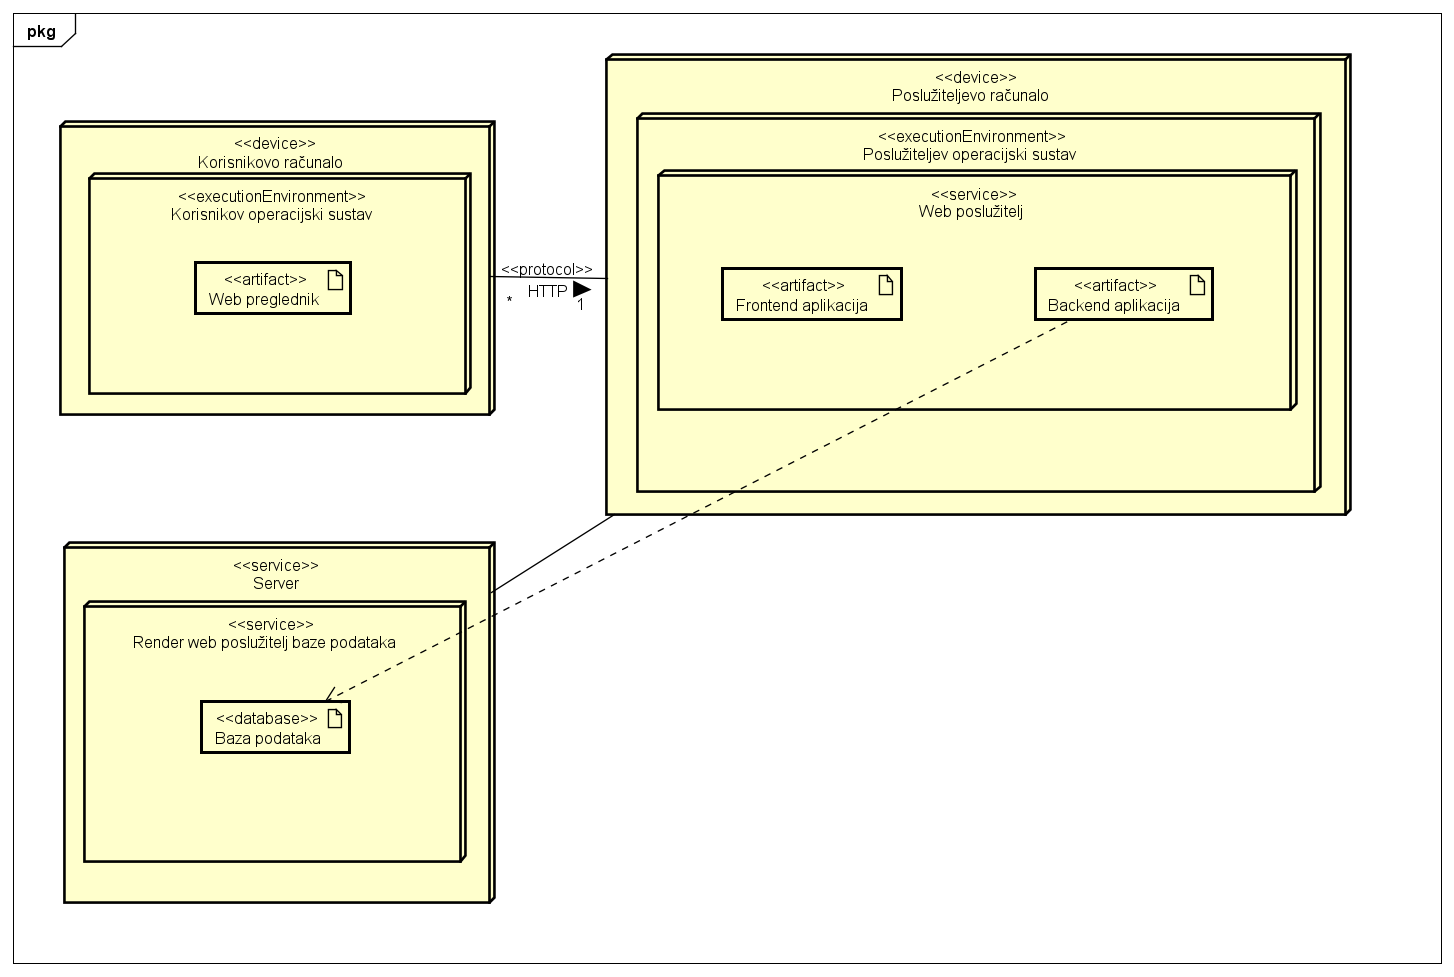
\includegraphics[width=1\textwidth]{slike/dijagrami/Dijagram razmjestaja.png}
				\caption{Dijagram razmještaja}
				\label{fig:enter-label}
			\end{figure}	

			\eject 
		
		\section{Upute za puštanje u pogon}
		
			\textbf{\textit{dio 2. revizije}}\\
		
			 \textit{U ovom poglavlju potrebno je dati upute za puštanje u pogon (engl. deployment) ostvarene aplikacije. Na primjer, za web aplikacije, opisati postupak kojim se od izvornog kôda dolazi do potpuno postavljene baze podataka i poslužitelja koji odgovara na upite korisnika. Za mobilnu aplikaciju, postupak kojim se aplikacija izgradi, te postavi na neku od trgovina. Za stolnu (engl. desktop) aplikaciju, postupak kojim se aplikacija instalira na računalo. Ukoliko mobilne i stolne aplikacije komuniciraju s poslužiteljem i/ili bazom podataka, opisati i postupak njihovog postavljanja. Pri izradi uputa preporučuje se \textbf{naglasiti korake instalacije uporabom natuknica} te koristiti što je više moguće \textbf{slike ekrana} (engl. screenshots) kako bi upute bile jasne i jednostavne za slijediti.}
			
			
			 \textit{Dovršenu aplikaciju potrebno je pokrenuti na javno dostupnom poslužitelju. Studentima se preporuča korištenje neke od sljedećih besplatnih usluga: \href{https://aws.amazon.com/}{Amazon AWS}, \href{https://azure.microsoft.com/en-us/}{Microsoft Azure} ili \href{https://www.heroku.com/}{Heroku}. Mobilne aplikacije trebaju biti objavljene na F-Droid, Google Play ili Amazon App trgovini.}
			
			
			\eject 